\chapter{The focused calculus}
% Before describing the calculus we must give some preliminary definitions

% Explaination on constraints why we use them ecc ecc ecc

\section{Normalization}\label{sec:normalization}
Since in linear logic negation is symmetric and an involution, it is usual to work only with formulae in negated normal form.
\begin{define}[Negated Normal Form -- NNF]
	\label{def:nnf}
	A formula is in NNF if all its linear implications ($\lolli$) are expanded to pars ($\llpar$) using the tautology
	$$ a \lolli b \Leftrightarrow \llnot{a} \llpar b$$
	and negation is pushed down to atoms.	% terms?
	Intuitively, a sequent is in NNF if all its formulae are in NNF.
\end{define}
A generic formula is then normalized applying recursively the DeMorgan rules for linear logic, until NNF is reached.
The process of normalization takes a two-sided judgment, of the form
$$ \Delta \vdash \Gamma $$
and transforms it into a one-sided judgment
$$ \vdash \Delta' $$
where the right side is composed of the normalization of $\Gamma$ and $\llnot{\Delta}$.

This choice has some implementation-wise advantages, but for now we will only care about the fact that it shrinks the size of the complete calculus by roughly half since we only have to deal with the right rules of the connectives.
\begin{figure}[H]
	\centering
	\begin{tblr}{ colspec = {cccccccccr}
		    , cells = { mode = math } 
		    % , vborder{1-4} = { leftspace = 0pt, rightspace = 0pt } 
		    }
		\phi & ::=  & 1              &\mid& \phi \llten \phi  &\mid& \bot &\mid& \phi \llpar \phi  & \text{(Multiplicatives and their constants)} \\
		     & \mid & 0              &\mid& \phi \llplus \phi &\mid& \top &\mid& \phi \llwith \phi & \text{(Additives and their constants)} \\
		     & \mid & \llbang{\phi}  &\mid& \llwn{\phi}       &    &      &    &                   & \text{(Exponentials)} \\
		     & \mid & \llnot{\alpha} &\mid& \alpha	      &    &      &    &                   & \text{(Where $\alpha$ is a term)}
	\end{tblr}
	\caption{Normalized linear logic formulae}
	\label{fig:ll-connectives}
\end{figure}
As seen in Figure \ref{fig:ll-connectives} we will use $\phi$ for formulae and $\alpha$ for terms.

\section{Focusing}
Focusing is a technique described by Andreoli in his seminal paper \cite{Focusing}.
There he recognizes two alternating phases in a proof: a deterministic phase, where the order of rule application to the sequent does not matter; and a non deterministic phase, where several choices may be tried.
These two phases are respectively called asynchronous and synchronous phase.
\begin{define}
	Given a formula $\phi$ we define the following predicates:
	``$\isAsy{\phi}$'' indicates that the rule for the top-level connective of the formula $\phi$ is asynchronous on the right, these connectives are 
	$$ \llpar\!, \llwith\!, \llwn{}, \lltop, \llbot $$
	conversely we define ``$\isSync{\phi}$'' to indicate that the rule for the top-level connective of $\phi$ is synchronous on the right, these are
	$$ \llten, \llplus, \llbang{}, \llone $$
\end{define}
Furthermore in focusing everything is assigned a negative or positive polarity.
Synchronous connectives are defined to have a positive polarity, whereas asynchronous connectives are define to have a negative polarity.
Terms also have a polarity, which may be assigned with some arbitrarily complex mechanisms.
We will follow \cite{LiangMiller} and simply assign atoms with a negative polarity and negated atoms with a positive one.
\begin{define}
	``$\isNegLit{\alpha}$'' is a predicate that is true only when $\alpha$ is a negative literal (i.e. an atom).
	Conversely ``$\isPosLit{\alpha}$'' is a predicate that is only when $\alpha$ is a positive literal (i.e. a negated atom).
\end{define}

\section{Constraints}

Our calculus uses constraints to manage the resources.
\begin{define}[Variables, expressions]
	\label{def:bool-expr}
	A boolean variable is simply a symbol to which one can associate a value of true or false.
	A boolean expression, in our case, is just a conjunction of possibly negated boolean variables.
\end{define}
\begin{define}[New variables]
	\label{def:new}
	Sometimes we will write 
	$$ \new{x}, \new{X} $$
	These mean respectively that:
	\begin{itemize}
		\item the variable name $x$ has not yet occurred in any expression in the proof tree, i.e. does not appear in any constraint of the father, or of its (the father) siblings and their sub-trees.
		\item each variable name $x_i, x_j \in X$ has not yet occurred in the proof and each variable in $X$ is distinct.
			$$ \forall i, j \mid i \neq j \Rightarrow x_i \neq x_j $$
	\end{itemize}
\end{define}
As seen in Figure \ref{fig:var-name} we will call $e$ such a conjunction and $x$ the single boolean variables.
\begin{figure}[h!]
	\centering
	\begin{tblr}{ colspec = {cccccr}, cells = { mode = math } }
		x & ::=  & x_i &\mid& \overline{x_i} & \text{(Variable)}\\
		e & ::=  & x \wedge e    &\mid& x & \text{(Expression)} \\
	\end{tblr}
	\caption{Definition of a boolean variable and expression}
	\label{fig:var-name}
\end{figure}

\begin{define}[Annotated formula]
	\label{def:annotated}
	Given a formula $\phi$ defined as in Figure \ref{fig:ll-connectives} and a boolean expression $e$ defined as in Definition \ref{def:bool-expr}, an \textit{annotated formula} is simply a term 
	$$ \af{\phi}{e} $$
	that associates the formula to the expression.
	We denote 
	\begin{itemize}
		\item $ \mathrm{exp}(\af{\phi}{e}) = e $
			as the operation of extracting the boolean expression associated to a given formula; and then extend this notation to sequents such that $ \mathrm{exp}(\Delta) $ is the set of all boolean expressions of $\Delta$.
		\item $\mathrm{vars}(\af{\phi}{e}) = \{ x_i \mid x_i \in e \} $
			as the operation of extracting the set of variables appearing in the expression $e$; and then extend this notation to sequents such that $ \mathrm{vars}(\Delta)$ is the set of all the variables appearing in the boolean expressions of the annotated formulae of $\Delta$.
	\end{itemize}
\end{define}
It is important to note that only the topmost connective gets annotated, and not the sub-formulae.

\noindent The purpose of putting formulae and expressions together in the annotated formula is twofold:
\begin{itemize}
	\item the actions taken on the formula determine the constraints that will be generated, and these depend on the variables associated to said formula;
	\item after the constraints are solved we can query the assignment of the variables and find out if the associated formula is used or not in a certain branch of a proof.
\end{itemize}
These constraints may be only of two kinds: ``$\avail{e}$'' and ``$\used{e}$''.
\begin{define}[Constraints]
	\label{def:constraints}
	Given an annotated formula $\af{\phi}{e}$ as in Definition \ref{def:annotated}, a constraint $\lambda$ may be of two kinds
	\begin{itemize}
		\item ``$\used{e}$'' states that the formula $\phi$ gets consumed in this branch of the proof.
			This corresponds to saying the expression $e$ is true or
			$$ x_i \wedge \dots \wedge x_j = \top $$
		\item ``$\avail{e}$'' states that the formula $\phi$ does not get consumed in this branch of the proof, and thus is available to be used in another branch.
			This corresponds to saying the expression $e$ is not true or
			$$ x_i \wedge \dots \wedge x_j = \bot $$
	\end{itemize}
	We then extend these predicates to sequents
	\begin{align*}
		\used{\Delta} &= \{ \used{e} \mid e \in \mathrm{exp}(\Delta) \} \\
		\avail{\Delta} &= \{ \avail{e} \mid e \in \mathrm{exp}(\Delta) \}
	\end{align*}
	We denote
	\begin{itemize}
		\item $\mathrm{exp}(\lambda) = e$ where $\lambda$ is either $\used{e}$ or $\avail{e}$;
		\item $\mathrm{vars}(\lambda) = \mathrm{vars}(\mathrm{exp}(\lambda))$, and extend this notation to a set of constraints $\Lambda$
			$$ \mathrm{vars}(\Lambda) = \bigcup_{\lambda \in \Lambda} \mathrm{vars}(\lambda) $$
	\end{itemize}
\end{define}
\begin{define}[Evaluation]
	Given a boolean expression $e$ and a function V mapping variables to their values 
	$$ \mathV : \{ x_1, x_2, \dots, x_n \} \rightarrow \{ \top, \bot \} $$
	with $\mathrm{vars}(e) \subseteq \mathrm{Dom}(\mathV)$; we write
		$$ e[\mathV] = e[\dots, x_i \subst \mathV(x_i), x_j \subst \mathV(x_j), \dots] $$
	as the value of the expression $e$ substituting with the assignment V.
	We extend this notation, such that
	\begin{itemize}
		\item given a constraint $\lambda$ and an assignment V, such that $\mathrm{vars}(\lambda) \subseteq \mathrm{Dom}(\mathV)$
			$$ 
			\begin{cases} 
				\used{e}[\mathV] = \top & \text{if } e[\mathV] = \top \\
				\used{e}[\mathV] = \bot & \text{if } e[\mathV] = \bot \\
				\avail{e}[\mathV] = \top & \text{if } e[\mathV] = \bot \\
				\avail{e}[\mathV] = \bot & \text{if } e[\mathV] = \top \\
			\end{cases}
			$$
		\item given an annotated sequent $\Delta$ and an assignment V, such that $\mathrm{vars}(\Delta) \subseteq \mathrm{Dom}(\mathV)$
			$$ \Delta[\mathV] = \{ \phi \mid \af{\phi}{e} \in \Delta , e[\mathV] = \top \} $$
	\end{itemize}
\end{define}
A branch is then considered as correct if its constraints are satisfiable.
Otherwise the branch of the proof fails.
\begin{define}[Satisfaiability of constraints]
	\label{def:sat}
	Given a set of constraints $\Lambda$ and an assignment function V with $\mathrm{vars}(\Lambda) \subseteq \mathrm{Dom}(\mathV)$; we write 
	$$ \sat{\Lambda}{\mathV} \Leftrightarrow \bigwedge_{\lambda \in \Lambda} \lambda[\mathV] = \top $$
\end{define}
\begin{fact}
	\label{fact:ass-trans}
	We can translate an assignment function to a set of constraints using simple reversible transformations:
	\begin{align*}
		\mathV &= \{ \dots, (x_i, \top), (x_j, \bot), \dots \} \\
		       &= \{ \dots, x_i = \top, x_j = \bot, \dots \} \\
		       &= \{ \dots, \used{x_i}, \avail{x_j}, \dots \}
	\end{align*}
\end{fact}

We now expand the concept of triadic sequent of \cite{Focusing} by adding constraints
\begin{define}[Members of the sequent]
	Given any sequent this can be in either two forms:
	\begin{itemize}
		\item focused or in the synchronous phase, written:
			$$\focus{\Psi}{\Delta}{\phi} \separator \constr{\Lambda}{\mathV}$$
		\item in the asynchronous phase, written:
			$$\async{\Psi}{\Delta}{\Phi} \separator \constr{\Lambda}{\mathV}$$
	\end{itemize}
	Where 
	\begin{itemize}
		\item $\Psi$ is a set of unrestricted formulae, or all formulae that can be freely discarded or duplicated;
		\item $\Delta$ and $\Phi$ are multisets of linear (annotated) formulae, these are respectively the formulas ``put to the side'' and the formulae which are being ``worked on'' during a certain moment of the asynchronous phase;
		\item $\Lambda$ and V are the constraints and the solution as defined in Definition \ref{def:sat}.
			By adding these members we make the flow of constraints through the proof tree explicit, leaving no ambiguity to where the constraints should be checked.
			This approach to constraints differs from the one in \cite{HarlandPym}, which prioritizes generality.
			The choice of letters is mainly a mnemonic or visual one, constraints $\Lambda$ ``go-up'' the proof tree and solutions V ``come down'' from the leaves.
	\end{itemize}
\end{define}

\begin{define}[Splitting]
	\label{def:split}
	Given a sequent of annotated formulae $\Delta$ and a set of variables $X$ such that $|\Delta| = |X|$ we define the operation of splitting it as a function
	$$ \mathrm{split}(\Delta, X) \mapsto (\Delta_L, \Delta_R) $$
	where
	\begin{align*}
		\Delta_L &= \{ \af{\phi_i}{x_i \wedge e_i} \mid i \in \{1, \dots, n\}\} \\
		\Delta_R &= \{ \af{\phi_i}{\varNot{x_i} \wedge e_i} \mid i \in \{1, \dots, n\}\}
	\end{align*}
	with $n$ the cardinality of $\Delta$, and $\phi_i$ (resp. $e_i$) the formula (resp. the expression) of the $i$-eth annotated formula in $\Delta$ using an arbitrary order.
	The same holds for $x_i$ and $X$.

	\noindent With a slight abuse of notation we will write $\Delta_L^X$ and $\Delta_R^X$ respectively as the left projection and the right projection of the pair $(\Delta_L, \Delta_R)$.
\end{define}
As a small example for clarity, given the sequent
\begin{align*}
	\Delta &= \af{a \llten b}{x_1}, \af{\llnot{c}}{x_2} \\
	X      &= \{ x_3, x_4 \} 
\end{align*}
this is split into
\begin{align*}
	\Delta_L^X &= \af{a \llten b}{x_3 \varAnd x_1}, \af{\llnot{c}}{x_4 \varAnd x_2} \\
	\Delta_R^X &= \af{a \llten b}{\varNot{x_3} \varAnd x_1}, \af{\llnot{c}}{\varNot{x_4} \varAnd x_2} 
\end{align*}
% example of splitting and variables

% One simple but important detail that will be useful later when explaining the Prolog implementation is noting that the variables in common between two branches with the same root are always introduced before the two branches diverge.
% Or -- put differently -- all new variables introduced in any point of a path from the root of the proof to a leaf may appear only in the subtrees.	% sistemo

We are now ready to present the full calculus.
\begin{figure}[H]
	\begin{subfigure}{\textwidth}
		\centering
			\begin{tblr}{ colspec = { cc }
				    , rows = {abovesep=7pt, belowsep=7pt}
				    }
			\SetCell[c=2]{c} {\footnotesize
			\AX$\async{\Psi}{\Delta}{\af{\phi_1}{e}, \af{\phi_2}{e}, \Phi} \fCenter \separator \constr{\Lambda, \used{e}}{\mathV}$
			\LeftLabel{$[\llpar]$}
			\UI$\async{\Psi}{\Delta}{\af{\phi_1 \llpar \phi_2}{e}, \Phi} \fCenter \separator \constr{\Lambda}{\mathV}$
			\DP} \\
			{\footnotesize
			\AX$\async{\Psi}{\Delta}{\Phi} \fCenter \separator \constr{\Lambda, \used{e}}{\mathV}$
			\LeftLabel{$[\llbot]$}
			\UI$\async{\Psi}{\Delta}{\af{\llbot}{e}, \Phi} \fCenter \separator \constr{\Lambda}{\mathV}$
			\DP}
			&
			{\footnotesize
			\AXC{}
			\LeftLabel{$[\lltop]$}
			\UIC{$\async{\Psi}{\Delta}{\af{\lltop}{-}, \Phi} \separator \constr{\Lambda}{\mathV}$}
			\DP
			}
			\\
			\SetCell[c=2]{c} {\footnotesize
			\AXC{$\async{\Psi}{\Delta}{\af{\phi_2}{e}, \Phi} \separator \constr{\Lambda, \used{e}}{\mathV'}$}
			\AXC{$\async{\Psi}{\Delta}{\af{\phi_1}{e}, \Phi} \separator \constr{\Lambda, \used{e}}{\mathV''}$}
			\LeftLabel{$[\llwith]$}
			\BIC{$\async{\Psi}{\Delta}{\af{\phi_1 \llwith \phi_2}{e}, \Phi} \separator \constr{\Lambda}{\mathV''}$}	
			\DP}
			\\
			\SetCell[c=2]{c} {\footnotesize
			\AX$\async{\phi, \Psi}{\Delta}{\Phi} \fCenter \separator \constr{\Lambda}{\mathV}$
			\LeftLabel{$[\,?\,]$}
			\UI$\async{\Psi}{\Delta}{\af{\llwn{\phi}}{-}, \Phi} \fCenter \separator \constr{\Lambda}{\mathV}$
			\DP} 
			\\
			\SetCell[c=2]{c} {\footnotesize
			\AXC{$\neg\isAsy{\phi}$}
			\AXC{$\async{\Psi}{\af{\phi}{e}, \Delta}{\Phi} \separator \constr{\Lambda}{\mathV}$}
			\LeftLabel{$[R\!\Uparrow]$}
			\BIC{$\async{\Psi}{\Delta}{\af{\phi}{e}, \Phi} \separator \constr{\Lambda}{\mathV}$}
			\DP
			}
		\end{tblr}
		\caption{Asynchronous rules}
	\end{subfigure}
\end{figure}
\begin{figure}[H]
	\ContinuedFloat
	\begin{subfigure}{\textwidth}
		\centering
		\begin{tblr}{ colspec = { cc } 
			    , rows = {abovesep=7pt, belowsep=7pt}
			    }
			\SetCell[c=2]{c} {\footnotesize
			\AXC{$ \new{X} \hspace{.3cm} 
				\focus{\Psi}{\Delta_L^X}{\af{\phi_1}{e}} \separator \constr{\Lambda, \used{e}}{\mathV'} \hspace{.3cm} 
				\focus{\Psi}{\Delta_R^X}{\af{\phi_2}{e}} \separator \constr{\mathV'}{\mathV''}$}
			\LeftLabel{$[\llten]$}
			\UIC{$\focus{\Psi}{\Delta}{\af{\phi_1 \llten \phi_2}{e}} \separator \constr{\Lambda}{\mathV''}$}	% capisco il movimento dei constraint
			\DP}
			\\ 
			{\footnotesize
			\AX$\focus{\Psi}{\Delta}{\af{\phi_1}{e}} \fCenter \separator \constr{\Lambda, \used{e}}{\mathV}$
			\LeftLabel{$[\llplus_L]$}
			\UI$\focus{\Psi}{\Delta}{\af{\phi_1 \llplus \phi_2}{e}} \fCenter \separator \constr{\Lambda}{\mathV}$
			\DP}
			&
			{\footnotesize
			\AX$\focus{\Psi}{\Delta}{\af{\phi_2}{e}} \fCenter \separator \constr{\Lambda, \used{e}}{\mathV}$
			\LeftLabel{$[\llplus_R]$}
			\UI$\focus{\Psi}{\Delta}{\af{\phi_1 \llplus \phi_2}{e}} \fCenter \separator \constr{\Lambda}{\mathV}$
			\DP}
			\\
			{\footnotesize
			\AXC{$\sat{ \Lambda, \used{e}, \avail{\Delta}}{\mathV}$}
			\LeftLabel{$[1]$}
			\UIC{$\focus{\Psi}{\Delta}{\af{\llone}{e}} \separator \constr{\Lambda}{\mathV}$}
			\DP} 
			&
			{\footnotesize
			\AX$\focus{\Psi}{\Delta}{\af{\phi}{e_1}} \fCenter \separator \constr{\Lambda, \used{e_1}, \avail{\Delta}}{\mathV}$
			\LeftLabel{$[\,!\,]$}
			\UI$\focus{\Psi}{\Delta}{\af{\llbang{\phi}}{e_1}} \fCenter \separator \constr{\Lambda}{\mathV}$
			\DP
			}
			\\
			\SetCell[c=2]{c} {\footnotesize
			\AXC{$\isAsy{\phi} \vee \isNegLit{\phi}$}
			\AXC{$\async{\Psi}{\Delta}{\af{\phi}{e}} \separator \constr{\Lambda}{\mathV}$}
			\LeftLabel{$[R\!\Downarrow]$}
			\BIC{$\focus{\Psi}{\Delta}{\af{\phi}{e}} \separator \constr{\Lambda}{\mathV}$}
			\DP
			}
		\end{tblr}
		\caption{Synchronous rules}
	\end{subfigure}
\end{figure}
\begin{figure}[H]
	\ContinuedFloat
	\begin{subfigure}{\textwidth}
		\centering
		\begin{tblr}{ colspec = { cc }
			    , rows = {abovesep=7pt, belowsep=7pt}
			    , vborder{1-2} = { leftspace = -5pt, rightspace = -5pt } 
			    }
			{\footnotesize
			\AXC{$ \isNegLit{\alpha} $}
			\AXC{$ \sat{\Lambda, \used{e_1}, \used{e_2}, \avail{\Delta}}{\mathV}$}
			\LeftLabel{$[I_1]$}
			\BIC{$\focus{\Psi}{\af{\alpha}{e_1}, \Delta}{\af{\llnot{\alpha}}{e_2}} \separator \constr{\Lambda}{\mathV}$}
			\DP}
			&
			{\footnotesize
			\AXC{$\neg \isNegLit{\phi}$}
			\AXC{$\focus{\Psi}{\Delta}{\af{\phi}{e}} \separator \constr{\Lambda}{\mathV}$}
			\LeftLabel{$[D_1]$}
			\BIC{$\async{\Psi}{\af{\phi}{e}, \Delta}{.} \separator \constr{\Lambda}{\mathV}$}
			\DP}
			\\
			{\footnotesize
			\AXC{$ \isNegLit{\alpha} $}
			\AXC{$ \sat{\Lambda, \used{e}, \avail{\Delta}}{\mathV}$}
			\LeftLabel{$[I_2]$}
			\BIC{$\focus{\alpha, \Psi}{\Delta}{\af{\llnot{\alpha}}{e}} \separator \constr{\Lambda}{\mathV}$}
			\DP}
			&
			{\footnotesize
			\AXC{$\neg \isNegLit{\phi}$}
			\AXC{$\new{x}$}
			\AXC{$\focus{\Psi}{\Delta}{\af{\phi}{x}} \separator \constr{\Lambda, \used{e}}{\mathV}$}
			\LeftLabel{$[D_2]$}
			\TrinaryInfC{$\async{\phi, \Psi}{\Delta}{.} \separator \constr{\Lambda}{\mathV}$}
			\DP}
		\end{tblr}
		\caption{Identity and decide rules}
	\end{subfigure}
	\caption{Focused constraint calculus for Linear Logic}
	\label{fig:calculus}
\end{figure}
What is described in Figure \ref{fig:calculus} is roughly the ``lazy'' strategy described by \cite{HarlandPym}.

\begin{lemma}
	\label{lemma:cap}
	Forall assignments $\mathV$ and sequents $\Delta$,
	$$ \Delta_L^X[\mathV] \cap \Delta_R^X[\mathV] = \varnothing $$
\end{lemma}
\begin{proof}
	This is a simple consequence of the fact that if $\phi \in \Delta_L^X[\mathV]$ there is a annotated formula $\af{\phi}{e} \in \Delta$ such that 
	$$ e[\mathV] = \top $$
	Since $e$ is defined as a conjunction on boolean variables, all the variables in it must be true.
	It is straightforward to see that if the variable added by the split in $\Delta_L^X$ is $x_i$, and the corresponding one in $\Delta_R^X$ is $\varNot{x_i}$, then when $x_i$ is true in the assignment V, $\llnot{x_i}$ is false.
	Hence $\phi \not \in \Delta_R^X[\mathV]$.
	The same can be done to show that if $\phi \in \Delta_R^X[\mathV]$ then $\phi \not \in \Delta_L^X[\mathV]$.
\end{proof}
\begin{lemma}
	\label{lemma:cup}
	Forall assignments $\mathV$ and sequents $\Delta$,
	$$ \Delta[\mathV] = \Delta_L^X[\mathV] \cup \Delta_R^X[\mathV] $$
\end{lemma}
\begin{proof}
	The simpler side is $\Delta_L^X[\mathV] \cup \Delta_R^X[\mathV] \subseteq \Delta[\mathV]$, since it  holds by the definition of the split (Definition \ref{def:split}).
	For the other side, suppose there was a formula $\phi$ such that $\phi \in \Delta[\mathV]$ and $\phi \not \in \Delta_L^X[\mathV] \cup \Delta_R^X[\mathV]$.
	This means that for some variable $x_i$ 
	\begin{align*}
		\af{\phi}{e} \in \Delta &\Rightarrow e[\mathV] = \top \\
		\af{\phi}{x_i \varAnd e} \not \in \Delta_L^X &\Rightarrow x_i \varAnd e[\mathV] = \bot \\
		\af{\phi}{\varNot{x_i} \varAnd e} \not \in \Delta_R^X &\Rightarrow \varNot{x_i} \varAnd e[\mathV] = \bot
	\end{align*}
	But either $x_i$ or $\varNot{x_i}$ must be true in a certain assignment, thus either $x_i \varAnd e$ or $\varNot{x_i} \varAnd e$ must be true, contradicting the hypothesis.
\end{proof}
\begin{lemma}
	Given any assignment $\mathV$ and any sequent $\Delta$, splitting induces a partition on the sequent $\Delta[\mathV]$.
\end{lemma}
\begin{proof}
	See Lemma \ref{lemma:cap} and \ref{lemma:cup}.
\end{proof}

\begin{lemma}
	\label{lemma:constr}
	Forall assignments $\mathV$ and set of constraints $\Lambda$, if (using the translation of Fact \ref{fact:ass-trans})
	$$ \sat{\mathV, \Lambda}{\mathV'} $$
	then $\mathrm{Dom}(\mathV) \subseteq \mathrm{Dom}(\mathV')$ and
	$$ \forall x_i \in \mathrm{Dom}(\mathV) \mid \mathV(x_i) = \mathV'(x_i) $$
	In this case we say that $\mathV'$ subsumes $\mathV$.
\end{lemma}
\begin{proof}
	The proof is straightforward: 
	\begin{itemize}
		\item the first condition trivially holds, since an assignment must be defined for each variable in the constraints and $\mathV'$ is an assignment defined for a superset of the constraints derived from V;
		\item for the second condition we have that
			$$ \mathV, \Lambda = \{ \dots, \used{x_i}, \avail{x_j}, \dots \} \cup \Lambda $$
		and to have that $ \sat{\mathV, \Lambda}{\mathV'} $
			$$ \bigwedge_{\lambda \in \mathV, \Lambda} \lambda[\mathV'] = \top $$
		thus the constraints derived from V must still hold with assignment $\mathV'$.
	\end{itemize}
\end{proof}
\begin{lemma}
	\label{lemma:subsume}
	Forall sets of constraints $\Lambda$ and forall assignments $\mathV$, if
	$$ \sat{\Lambda}{\mathV} $$
	then for any $\Lambda' \subseteq \Lambda$
	$$ \sat{\Lambda'}{\mathV} $$
\end{lemma}
\begin{proof}
	Following the Definition \ref{def:sat} of satisfiability, every constraint in $\Lambda$ must hold under assignment $\mathV$.
	This trivially means that all the constraints in $\Lambda'$ must also hold.
\end{proof}

\begin{teor}[Soundness]\label{thm:soundness}
	% Let $\vdash \Psi$ The calculus of Figure \ref{fig:calculus} is sound % ...
\end{teor}
\begin{proof}
	As a soundness proof we give a translation to the triadic system defined by Andreoli in \cite{Focusing}:
	\begin{figure}[H]
		\centering
		\begin{tblr}{ colspec = {c c c}
			, cells = { mode = dmath } 
			, rows = {abovesep=7pt, belowsep=7pt}
			, vborder{1-2} = { leftspace = -5pt, rightspace = -5pt } 
			}
			\AXC{$\async{\Psi}{\Delta}{\Phi}$}
			\LeftLabel{$[\llbot]$}
			\UIC{$\async{\Psi}{\Delta}{\llbot, \Phi}$}
			\DP
			&
			\AXC{$\async{\Psi}{\Delta}{\phi_1, \phi_2, \Phi}$}
			\LeftLabel{$[\llpar]$}
			\UIC{$\async{\Psi}{\Delta}{\phi_1 \llpar \phi_2, \Phi}$}
			\DP
			&
			\AXC{$\async{\phi, \Psi}{\Delta}{\Phi}$}
			\LeftLabel{$[\llwn{}]$}
			\UIC{$\async{\Psi}{\Delta}{\llwn{\phi}, \Phi}$}
			\DP
			\\
			\AXC{}
			\LeftLabel{$[\lltop]$}
			\UIC{$\async{\Psi}{\Delta}{\lltop, \Phi}$}
			\DP
			&
			\SetCell[c=2]{c} 
			\AXC{$\async{\Psi}{\Delta}{\phi_1, \Phi}$}
			\AXC{$\async{\Psi}{\Delta}{\phi_2, \Phi}$}
			\LeftLabel{$[\llwith]$}
			\BIC{$\async{\Psi}{\Delta}{\phi_1 \llwith \phi_2, \Phi}$}
			\DP
			\\
			\AXC{$\focus{\Psi}{\Delta}{\phi_1}$}
			\LeftLabel{$[\llplus_L]$}
			\UIC{$\focus{\Psi}{\Delta}{\phi_1 \llplus \phi_2}$}
			\DP
			&
			\AXC{}
			\LeftLabel{$[\llone]$}
			\UIC{$\focus{\Psi}{.}{\llone}$}
			\DP
			& 
			\AXC{$\async{\Psi}{.}{\phi}$}
			\LeftLabel{$[\llbang{}]$}
			\UIC{$\focus{\Psi}{.}{\llbang{\phi}}$}
			\DP
			\\
			\AXC{$\focus{\Psi}{\Delta}{\phi_2}$}
			\LeftLabel{$[\llplus_R]$}
			\UIC{$\focus{\Psi}{\Delta}{\phi_1 \llplus \phi_2}$}
			\DP
			&
			\SetCell[c=2]{c} 
			\AXC{$\focus{\Psi}{\Gamma}{\phi_1}$}
			\AXC{$\focus{\Psi}{\Delta}{\phi_2}$}
			\LeftLabel{$[\llten]$}
			\BIC{$\focus{\Psi}{\Gamma, \Delta}{\phi_1 \llten \phi_2}$}
			\DP
			\\
			\AXC{$\neg \isAsy{\phi}$}
			\AXC{$\async{\Psi}{\phi, \Delta}{\Phi}$}
			\LeftLabel{$[R\!\Uparrow]$}
			\BIC{$\async{\Psi}{\Delta}{\phi, \Phi}$}
			\DP
			&
			\AXC{$\isNegLit{\alpha}$}
			\LeftLabel{$[I_1]$}
			\UIC{$\focus{\Psi}{\alpha}{\llnot{\alpha}}$}
			\DP
			&
			\AXC{$\focus{\Psi}{\Delta}{\phi}$}
			\LeftLabel{$[D_1]$}
			\UIC{$\async{\Psi}{\phi, \Delta}{.}$}
			\DP
			\\
			\AXC{$\isAsy{\phi} \vee \isNegLit{\phi}$}
			\AXC{$\async{\Psi}{\Delta}{\phi}$}
			\LeftLabel{$[R\!\Downarrow]$}
			\BIC{$\focus{\Psi}{\Delta}{\phi}$}
			\DP
			&
			\AXC{$\isNegLit{\alpha}$}
			\LeftLabel{$[I_2]$}
			\UIC{$\focus{\alpha, \Psi}{.}{\llnot{\alpha}}$}
			\DP
			&
			\AXC{$\focus{\Psi}{\Delta}{\phi}$}
			\LeftLabel{$[D_2]$}
			\UIC{$\async{\phi, \Psi}{\Delta}{.}$}
			\DP
		\end{tblr}
		\caption{J.-M. Andreoli's triadic calculus.}
		\label{fig:triadic}
	\end{figure}
	The three base cases are proved essentially in the same way:
	\begin{itemize}
		\item[$I_1$:] Given the judgment
			$$
			\AXC{$\isNegLit{\alpha}$}
			\AXC{$ \sat{\Lambda, \used{e_1}, \used{e_2}, \avail{\Delta}}{\mathV}$}
			\LeftLabel{$[I_1]$}
			\BIC{$\focus{\Psi}{\Delta, \af{\alpha}{e_1}}{\af{\llnot{\alpha}}{e_2}} \separator \constr{\Lambda}{\mathV}$}
			\DP
			$$
			looking at the constraints we trivially get that
			\begin{align*}
				\Delta[\mathV] &= . \tag{Because of $\avail{\Delta}$} \\
				\af{\alpha}{e_1}[\mathV] &= \alpha \tag{Because of $\used{e_1}$} \\
				\af{\llnot{\alpha}}{e_2}[\mathV] &= \llnot{\alpha} \tag{Because of $\used{e_2}$}
			\end{align*}
			so we can rewrite this as
			$$
			\AXC{$\isNegLit{\alpha}$}
			\LeftLabel{$[I_1]$}
			\UIC{$\focus{\Psi}{\alpha}{\llnot{\alpha}}$}
			\DP
			$$
		\item[$I_2$:] Given the judgment
			$$
			\AXC{$\isNegLit{\alpha}$}
			\AXC{$ \sat{\Lambda, \used{e}, \avail{\Delta}}{\mathV}$}
			\LeftLabel{$[I_2]$}
			\BIC{$\focus{\Psi, \alpha}{\Delta}{\af{\llnot{\alpha}}{e}} \separator \constr{\Lambda}{\mathV}$}
			\DP
			$$
			proceeding as above we get
			\begin{align*}
				\Delta[\mathV] &= . \\
				\af{\llnot{\alpha}}{e}[\mathV] &= \llnot{\alpha}
			\end{align*}
			thus
			$$
			\AXC{$\isNegLit{\alpha}$}
			\LeftLabel{$[I_2]$}
			\UIC{$\focus{\alpha, \Psi}{.}{\llnot{\alpha}}$}
			\DP
			$$
		\item[$\llone$:] Given the judgment
			$$
			\AXC{$\sat{ \Lambda, \used{e}, \avail{\Delta}}{\mathV}$}
			\LeftLabel{$[1]$}
			\UIC{$\focus{\Psi}{\Delta}{\af{\llone}{e}} \separator \constr{\Lambda}{\mathV}$}
			\DP
			$$
			proceeding as above we get
			\begin{align*}
				\Delta[\mathV] &= . \\
				\af{\llone}{e}[\mathV] &= \llone
			\end{align*}
			thus
			$$
			\AXC{}
			\LeftLabel{$[\llone]$}
			\UIC{$\focus{\Psi}{.}{\llone}$}
			\DP
			$$
	\end{itemize}
	The induction step is rather mechanic, with the exception of 
	\begin{itemize}
		\item the tensor rule ($\llten$):
			$$
			\AXC{$ \new{X} \hspace{.3cm} 
			\focus{\Psi}{\Delta_L^X}{\af{\phi_1}{e}} \separator \constr{\Lambda, \used{e}}{\mathV'} \hspace{.3cm} 
			\focus{\Psi}{\Delta_R^X}{\af{\phi_2}{e}} \separator \constr{\mathV'}{\mathV''}$}
			\LeftLabel{$[\llten]$}
			\UIC{$\focus{\Psi}{\Delta}{\af{\phi_1 \llten \phi_2}{e}} \separator \constr{\Lambda}{\mathV''}$}	% capisco il movimento dei constraint
			\DP
			$$
			By the Lemma \ref{lemma:constr} we can say that $\Delta_L^X[\mathV'] = \Delta_L^X[\mathV'']$, since $\mathV''$ subsumes $\mathV'$.
			This being said, using Lemma \ref{lemma:cap} we have that $\Delta_L^X[\mathV'']$ and $\Delta_R^X[\mathV'']$ are disjoint, so the contexts of the two branches are separated.
			Finally Lemma \ref{lemma:cup} guarantees that the union of the two contexts returns the whole original context.
			Given this we get that this equals to 
			$$
			\AXC{$\focus{\Psi}{\Delta_L^X[\mathV'']}{\phi_1}$}
			\AXC{$\focus{\Psi}{\Delta_R^X[\mathV'']}{\phi_2}$}
			\LeftLabel{$[\llten]$}
			\BIC{$\focus{\Psi}{\Delta_L^X[\mathV''], \Delta_R^X[\mathV'']}{\phi_1 \llten \phi_2}$}
			\DP
			$$
		\item the with rule ($\llwith$):
			$$
			\AXC{$\async{\Psi}{\Delta}{\af{\phi_2}{e}, \Phi} \separator \constr{\Lambda, \used{e}}{\mathV'}$}
			\AXC{$\async{\Psi}{\Delta}{\af{\phi_1}{e}, \Phi} \separator \constr{\Lambda, \used{e}}{\mathV''}$}
			\LeftLabel{$[\llwith]$}
			\BIC{$\async{\Psi}{\Delta}{\af{\phi_1 \llwith \phi_2}{e}, \Phi} \separator \constr{\Lambda}{\mathV''}$}
			\DP
			$$
			which after erasing the unused formulae using the assignment becomes
			$$
			\AXC{$\async{\Psi}{\Delta[\mathV']}{\phi_2, \Phi[\mathV']}$}
			\AXC{$\async{\Psi}{\Delta[\mathV'']}{\phi_1, \Phi[\mathV'']}$}
			\LeftLabel{$[\llwith]$}
			\BIC{$\async{\Psi}{\Delta[\mathV'']}{\phi_1 \llwith \phi_2, \Phi[\mathV'']}$}
			\DP
			$$
			or equivalently 
			$$
			\AXC{$\async{\Psi}{\Delta[\mathV']}{\phi_2, \Phi[\mathV']}$}
			\AXC{$\async{\Psi}{\Delta[\mathV'']}{\phi_1, \Phi[\mathV'']}$}
			\LeftLabel{$[\llwith]$}
			\BIC{$\async{\Psi}{\Delta[\mathV']}{\phi_1 \llwith \phi_2, \Phi[\mathV']}$}
			\DP
			$$
			since  $\Lambda \subseteq \used{e}, \Lambda$ and Lemma \ref{lemma:subsume}.
	\end{itemize}
	The rest of the translations are just a matter of canceling out the members of the sequent using the assignment function.
	\begin{center}
		\begin{tblr}{ colspec = { ccc }
			    , cells = { mode = dmath } 
			    , rows = {abovesep=5pt, belowsep=5pt}
			    }
			\llbot
			& \mapsto
			& 
			\AXC{$\async{\Psi}{\Delta[\mathV]}{\Phi[\mathV]}$}
			\UIC{$\async{\Psi}{\Delta[\mathV]}{\llbot, \Phi[\mathV]}$}
			\DP
			\\
			\llpar
			& \mapsto
			& 
 			\AXC{$\async{\Psi}{\Delta[\mathV]}{\phi_1, \phi_2, \Phi[\mathV]}$}
 			\UIC{$\async{\Psi}{\Delta[\mathV]}{\phi_1 \llpar \phi_2, \Phi[\mathV]}$}
 			\DP
			\\
			\llplus_L
			& \mapsto
			& 
 			\AXC{$\focus{\Psi}{\Delta[\mathV]}{\phi_1}$}
 			\UIC{$\focus{\Psi}{\Delta[\mathV]}{\phi_1 \llplus \phi_2}$}
 			\DP
			\\
			\llplus_R
			& \mapsto
			& 
 			\AXC{$\focus{\Psi}{\Delta[\mathV]}{\phi_2}$}
 			\UIC{$\focus{\Psi}{\Delta[\mathV]}{\phi_1 \llplus \phi_2}$}
 			\DP
			\\
			\llbang{}
			& \mapsto
			& 
 			\AXC{$\async{\Psi}{.}{\phi}$}
 			\UIC{$\focus{\Psi}{.}{\llbang{\phi}}$}
 			\DP
			\\
			\llwn{}
			& \mapsto
			&
 			\AXC{$\async{\phi, \Psi}{\Delta[\mathV]}{\Phi[\mathV]}$}
 			\UIC{$\async{\Psi}{\Delta[\mathV]}{\llwn{\phi}, \Phi[\mathV]}$}
 			\DP
			\\
			R \!\Downarrow 
			& \mapsto
			& 
 			\AXC{$\isAsy{\phi} \vee \isNegLit{\phi}$}
 			\AXC{$\async{\Psi}{\Delta[\mathV]}{\phi}$}
 			\BIC{$\focus{\Psi}{\Delta[\mathV]}{\phi}$}
 			\DP
			\\
			R\!\Uparrow 
			& \mapsto
			& 
 			\AXC{$\neg \isAsy{\phi}$}
 			\AXC{$\async{\Psi}{\phi, \Delta[\mathV]}{\Phi[\mathV]}$}
 			\BIC{$\async{\Psi}{\Delta[\mathV]}{\phi, \Phi[\mathV]}$}
 			\DP
			\\
			D_1
			& \mapsto
			& 
 			\AXC{$\focus{\Psi}{\Delta[\mathV]}{\phi}$}
 			\UIC{$\async{\Psi}{\phi, \Delta[\mathV]}{.}$}
 			\DP
			\\
			D_2
			& \mapsto
			& 
			\AXC{$\focus{\Psi}{\Delta[\mathV]}{\phi}$}
	 		\UIC{$\async{\phi, \Psi}{\Delta[\mathV]}{.}$}
 			\DP
			\\
			I_1
			& \mapsto
			& 
			\AXC{$\isNegLit{\alpha}$}
			\UIC{$\focus{\Psi}{\alpha}{\llnot{\alpha}}$}
			\DP
			\\
			I_2
			& \mapsto
			& 
			\AXC{$\isNegLit{\alpha}$}
			\UIC{$\focus{\alpha, \Psi}{.}{\llnot{\alpha}}$}
			\DP
		\end{tblr}
	\end{center}
		%	\item[$\lltop$:]
		%		$$
		%		\AXC{}
		%		\LeftLabel{$[\lltop]$}
		%		\UIC{$\async{\Psi}{\Delta}{\af{\lltop}{-}, \Phi} \separator \constr{\Lambda}{\mathV}$}
		%		\DP
		%		$$
\end{proof}

\begin{figure}[h!]
	\centering
	\begin{subfigure}{\textwidth}
		\centering
		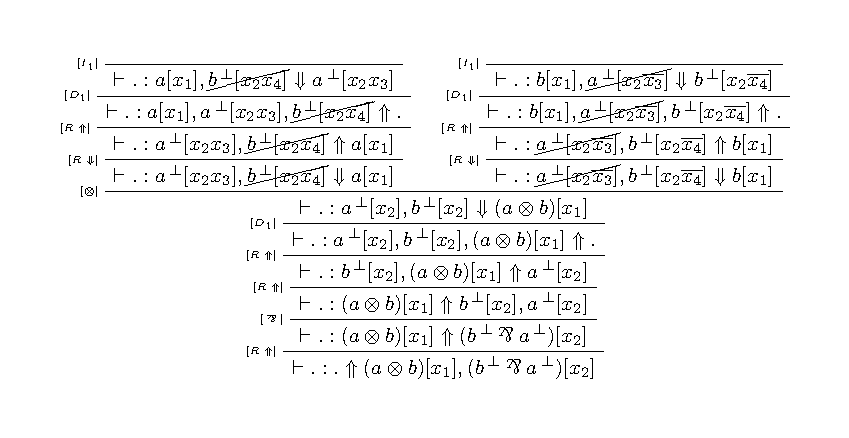
\includegraphics{./images/tensor_de_morgan_constr}
	\end{subfigure}
	\begin{subfigure}{\textwidth}
		\centering
		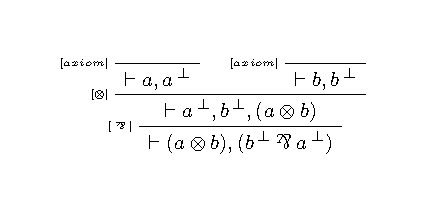
\includegraphics{./images/tensor_de_morgan_classic}
	\end{subfigure}
\end{figure}

